\documentclass[12pt,a4paper]{article}
\usepackage[utf8]{inputenc}
\usepackage[english,russian]{babel}
\usepackage{indentfirst}
\usepackage{misccorr}
\usepackage{graphicx}
\usepackage{amssymb}
\usepackage{amsmath}

\begin{document}

\begin{center}
    \large
    Работа 1.4.2
    
    Сибгатуллин Булат, Б01-007
    
    \vspace{0.5cm}
    \textbf{Изучение колебаний струны}

\end{center}

\vspace{0.5cm}
\textbf{Цель работы:} исследование зависимости частоты колебаний струны от величины натяжения, а также условий установления стоячей волны, получающейся в результате сложения волн, идущих в противоположных направлениях.
    
\vspace{0.5cm}
\textbf{В работе используются:} рейка со струной, звуковой генератор, постоянный магнит, разновесы. 

\vspace{0.5cm}

Изучения колебательных процессов удобно проводит с использованием натянутой струны с жестко закрепленными концами. Движение элементов струны может быть вызвано изменением ее формы или передачей ей импульса. Натяжение струны стремится вернуть ее в начальное положение и это приводит к тому, что возникает движение элементов струны. Возмущения бегут вдоль струны.

В силу волнового уравнения скорость распространения поперечной волны на струне равна:

\begin{equation}
u = \sqrt{\frac{F}{\rho_t}},
\end{equation}

где \textit{F} - сила натяжения струны, $\rho_t$ - масса струны на единицу длины. При заданной частоте $\nu$длина волны:

\begin{equation}
\lambda = \frac{u}{\nu}.
\end{equation}

Частоты собственных колебаний струны определяются формулой:

\begin{equation}
\nu_n = n \frac{u}{2l},
\end{equation}

где \textit{l} - длина струны, \textit{n} - число полуволн.

\begin{figure}[h!]
\centering
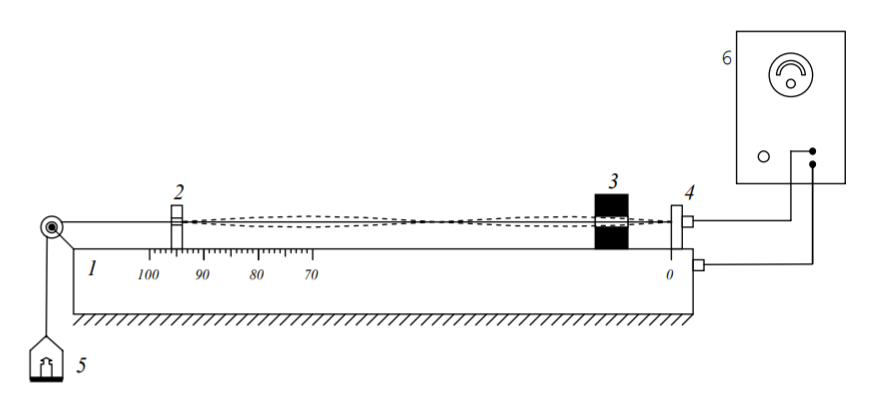
\includegraphics[scale=1]{setup.png}
\caption{Схема экспериментальной установки}
\label{fig:setup}
\end{figure}

\vspace{0.5cm}

\textbf{Экспериментальная установка (рис. 1).} По массивной металлической рейке 1 установлены опора 2 и магнит 3, которые можно перемещать вдоль рейки, а также неподвижная опора 4. Струна закреплена в изоляторе опоры 4 (один ее конец),проходеит между полюсами магнита и через опору 2, которая дает струне возможность перемещаться в горизонтальном напрвлении, неподвижный блок соединяется с чашкой 5, на которую помещают грузы. К концу струны, закрепленному на изоляторе опоры 4, и к массивной металлической рейке 1 подводится переменное напряжение от звукового генератора 6. Движение струны вызывается силой Ампера действующей на проводник с током в магнитном поле.
 
Так как в реальных условиях колебания струны существуют потерии энергии, то чтобы колебания струны происходили долго, нужно подводить энергию. В стационарном режиме подводимая энергия равна потерям энергии. В данной установке сила Ампера не только возбуждает, но и поддерживает колебания в струне.

Поток энергии распространяется при этом по всей струне. Однако в чисто стоячей волне распространение энергии невозможно. Наличие отличного от нуля коэффициента бегучести поэтому принципиально. Реально это приводит к размытию узлов стоячей волны. Если потери энергии за период колебаний малы по сравнению с запасом колебательной энергии в системе, то коэффициент бегучести значительно меньше единицы:

\begin{equation}
\frac{A_1 - A_2}{A_2} \ll 1.
\end{equation}

Здесь $A_1$ - амплитуда падающей волны, $A_2$ - амплитуда отраженной волны. В этом случае можно пользоваться соотношениями,полученными для чисто стоячей волны. Заметим, что величину $A_1 - A_2$ можно оценить по размытию узлов стоячей волны, она равна половине величины размытия. Амплитуда стоячей волны в пучности равна $2A_2$.

Если соотношение (4) выполняется недостаточно хорошо, то надо уменьшить величину подводимой от генератора энергии. При этом уменьшение потерь энергии происходит быстрее, чем уменьшение энергии в волне.

\vspace{0.5cm}

\textbf{Ход работы:}

1. Установить опору 2, так чтобы колеблющийся участок струны имел длину \textit{L} не менее 80 см.

2. Включить питание звукового генератора. Дать ему прогреться 5 - 10 минут.

3. Установить нулевое значение частот генератора (лимбы "Частота" и "Расстройка" установить на нуль). Вращая ручку "Установка нуля" устранить биение стрелки.

4. Нагрузить струну.

5. Перемещая магнит и вращая ручку изменения частоты генератора получить картину стоячих волн.

6. Увеличивая частоту звукового генератора при некотором постоянном натяжении струны, получить стоячие волны, соответсвтвуюшие \textit{n} = 1, 2, 3, ... , дойдя по крайней мере, до \textit{n} = 6. Повторить процесс при повышении и понижении частот. Проделать данные измерения при различных натяжениях струны.

7. При проведении эксперимента должно выполняться условие (4). Если оно не выполняется, надо уменьшить выходную мощность звукового генератора.

8. Для каждого значения натяжения струны \textit{F} постройте график зависимости частоты резонанса $\nu_n$ от \textit{n}. По наклону прямой определить скорость \textit{u} волн в струне при данном натяжении. Оценить погрешность результатов.

9. Построить график зависимости $u^2$ от $F$. По наклону прямой определить погонную плотность струны $\rho_t$. Оценить погрешность результата и сравнить оценку с действительной погрешностью.

\end{document}